\documentclass{article}
\usepackage{amsfonts, amsmath, amssymb, amsthm} % Math notations imported
\usepackage{enumitem}
\usepackage{graphicx}
\usepackage{setspace}
\usepackage{indentfirst}
\usepackage[margin=1in]{geometry}
\graphicspath{{./images/}} % Path to images

% \begin{figure}[htb!]
%      \centering
%      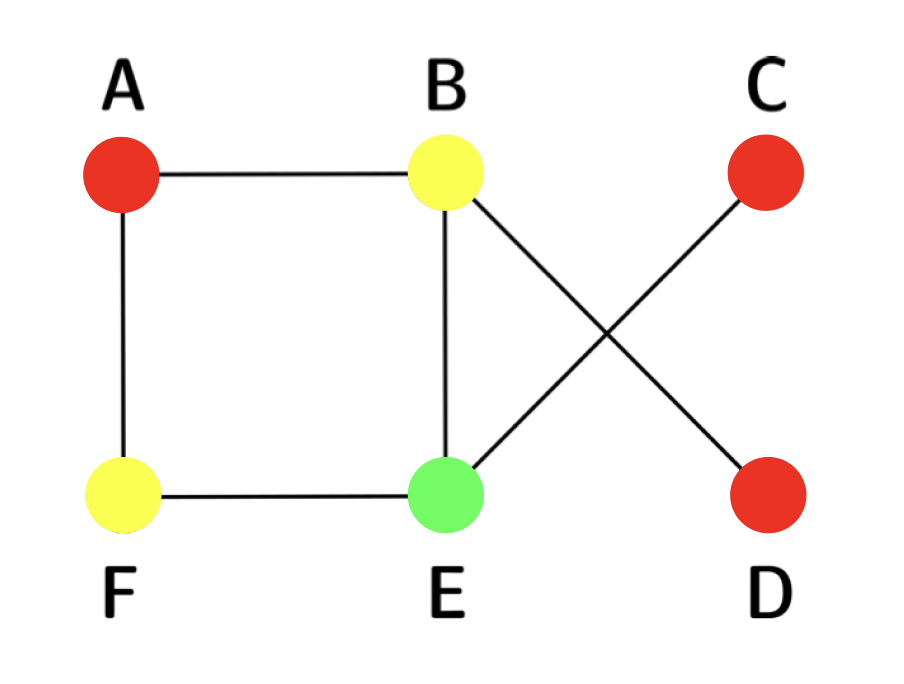
\includegraphics[scale=0.5]{coloring.png}
%      \caption{Coloring of the graph.}
% \end{figure}

% \begin{figure}[htb]
%     \qquad
%     \begin{minipage}{.4\textwidth}
%         \centering
%         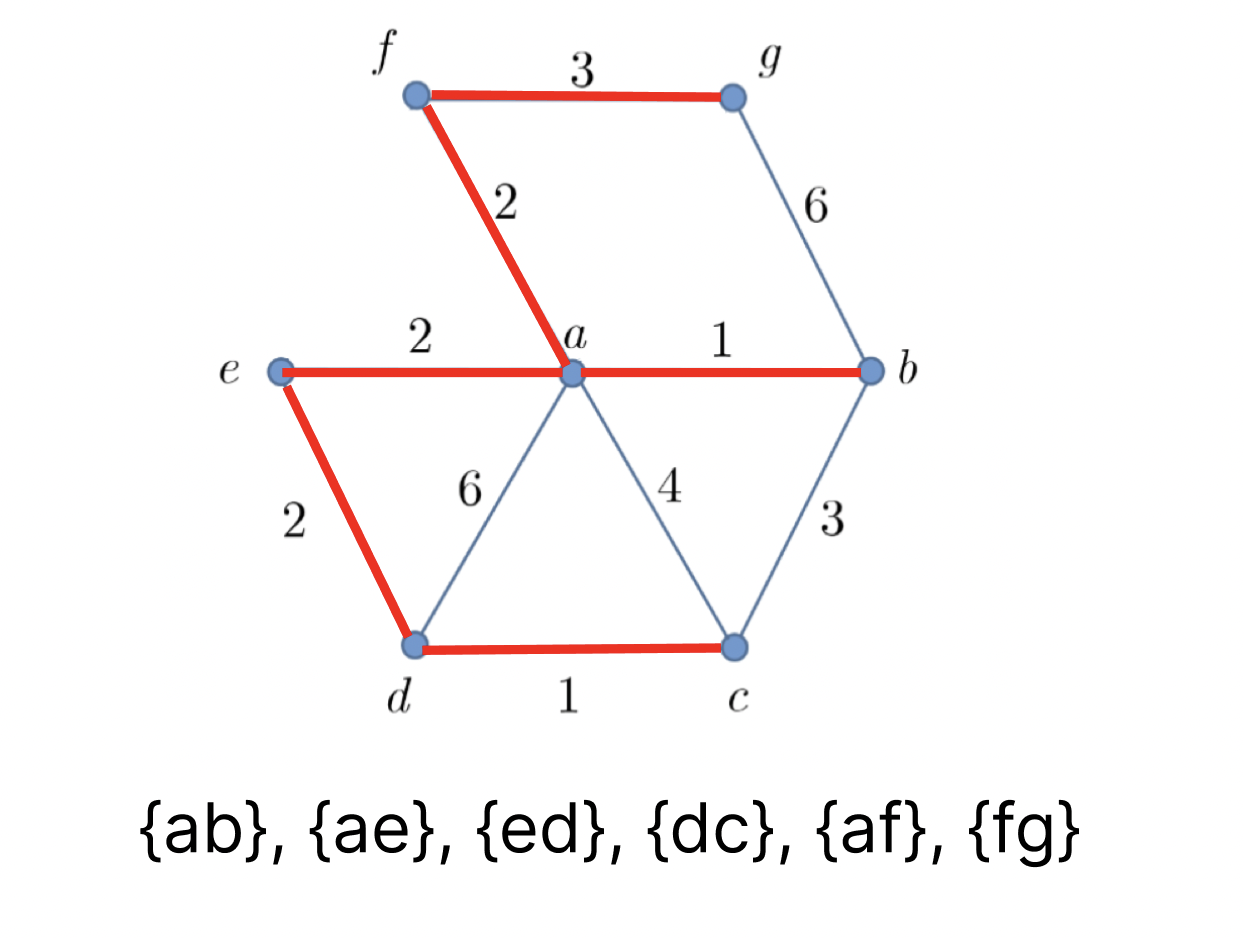
\includegraphics[scale=0.35]{prims.png}
%         \caption{}
%     \end{minipage}    
%     \qquad
%     \begin{minipage}{.4\textwidth}
%         \centering
%         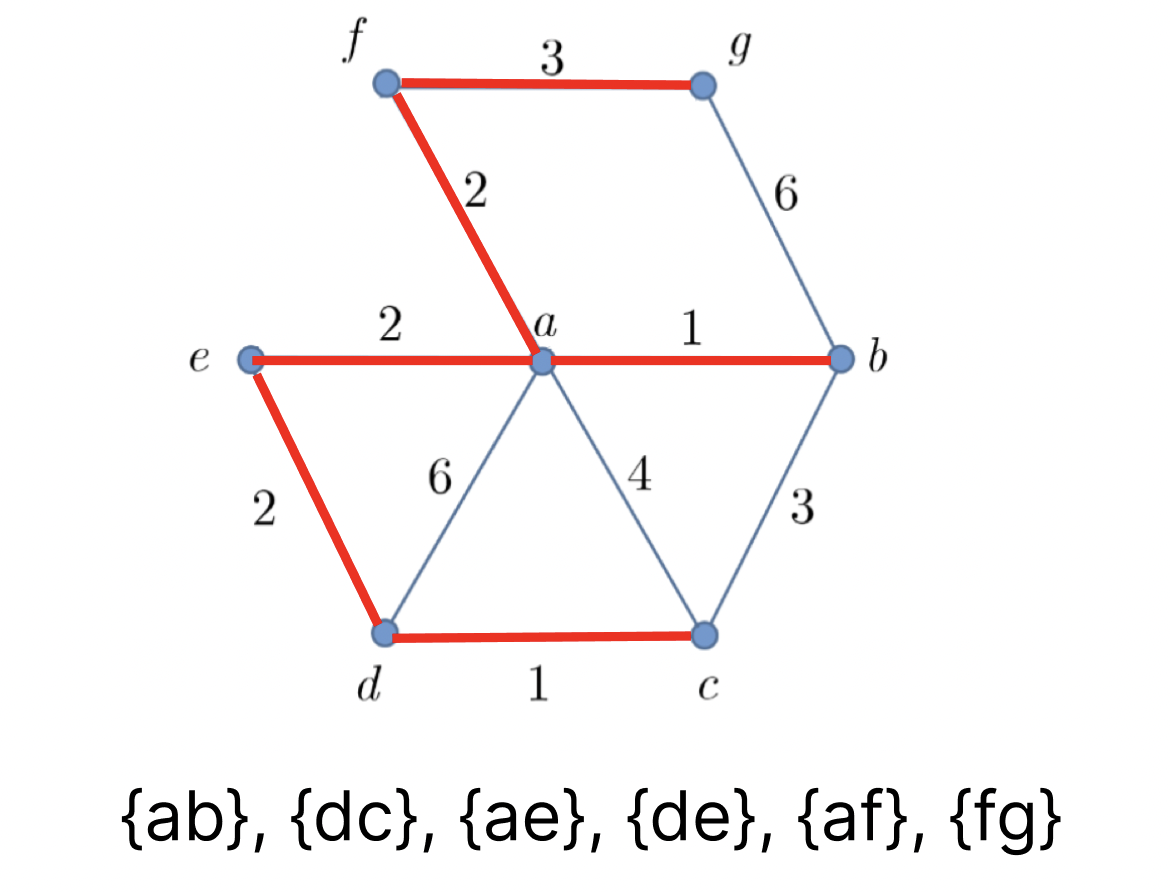
\includegraphics[scale=0.35]{kruskal.png}
%         \caption{}
%     \end{minipage}        
% \end{figure} 

\newtheorem{thm}{Theorem}
\newtheorem{proposition}[thm]{Proposition}
\newtheorem{cor}[thm]{Corollary}

% title information
\title{Math 104 HW5}
\author{Neo Lee}
\date{10/06/2023}

\setstretch{1.15}
% main content
\begin{document} 

% placing title information; comment out if using fancyhdr
\maketitle 

\subsection*{Exercise 11.3}
Consider the sequences
$$s_n=\cos\left(\frac{n\pi}{3}\right), \qquad t_n=\frac{3}{4n+1}, \qquad 
u_n=\left(-\frac{1}{2}\right)^n, \qquad v_n=(-1)^n+\frac{1}{n}.$$
\begin{enumerate}[label=(\alph*)]
    \item For each sequence, give an example of a monotone subsequence.
    \begin{proof}[Solution]\indent
        \begin{enumerate}
            \item[($s_n$):] Consider $n_k = 6k$ for $k\in\mathbb{N}$, then $s_{n_k} = 
            \cos\left(\frac{6k\pi}{3}\right)=\cos\left(2k\pi\right)=1$ for all $n_k$, which is 
            indeed monotone [a constant sequence is monotone].
            \item[($t_n$):] Consider $n_k = 2k$ for $k\in\mathbb{N}$, then $t_{n_k} =
            \frac{3}{8k+1}$ for all $n_k$, which is apparently monotonically decreasing.
            \item[($u_n$):] Consider $n_k = 2k$ for $k\in\mathbb{N}$, then $u_{n_k} =
            \left(-\frac{1}{2}\right)^{2k}=\frac{1}{4^k}$ for all $n_k$, which is apparently 
            monotonically decreasing.
            \item[($v_n$):] Consider $n_k = 2k$ for $k\in\mathbb{N}$, then $v_{n_k} =
            (-1)^{2k}+\frac{1}{2k}=1+\frac{1}{2k}$ for all $n_k$, which is apparently monotonically 
            decreasing.
        \end{enumerate}

    \end{proof}
    \item For each sequence, give its set of subsequential limits.
    \begin{proof}[Solution]\indent
        \begin{enumerate}
            \item[($s_n$):] $\{1, 0.5, -0.5, -1\}$. The values of $s_n$ oscillates among constant values
            $\{1, 0.5, -0.5, -1\}$. We can construct the constant subsequences, which have the limits 
            $1, 0.5, -0.5, -1$ respectively. Then consider any $x\not\in\{1, 0.5, -0.5, -1\}$, 
            any subsequence will have a minimum non-zero distance from $x$, hence unable to converge 
            to $x$. Therefore, the set of subsequential limits is $\{1, 0.5, -0.5, -1\}$.
            \item[($t_n$):] $\{0\}$. $\lim t_n=0$ by Theorem 9.3 - 9.6, hence the set of 
            subsequential limits only contains $\lim t_n=0$
            \item[($u_n$):] $\{0\}$. $\lim v_n=0$ by Theorem 9.7, hence the set of subsequential 
            limits only contains $\lim v_n=0$
            \item[($v_n$):] $\{1, -1\}$. Take only even $n$, then the subsequence converges to $1$.
            Take only odd $n$, then the subsequence converges to $-1$. Then consider any 
            subsequence with finite odd $n$, it will converge to $1$, just like the only even $n$ 
            subsequence because we can take $N$ larger than the finite odd $n$. Similarly, any
            subsequence with finite even $n$ will converge to $-1$. Finally, any subsequence 
            with infinite odd and even $n$ do not converge because it will always have elements 
            within the neighborhood of $1$ and $-1$. 
        \end{enumerate}
    \end{proof}

    \item For each sequence, give its $\lim \sup$ and $\lim \inf$.
    \begin{proof}[Solution]\indent
        Notice $\lim \sup x_n = \sup S$ and $\lim \inf x_n = \inf S$, where $x_n$ is any arbitrary 
        sequence.
        \begin{enumerate}
            \item[($s_n$):] $\lim \sup s_n = 1, \lim \inf s_n = -1$. 
            \item[($t_n$):] $\lim \sup t_n = \lim \inf t_n = 0$.
            \item[($u_n$):] $\lim \sup u_n = \lim \inf u_n = 0$.
            \item[($v_n$):] $\lim \sup v_n=1, \lim\inf v_n=-1$. 
        \end{enumerate}
    \end{proof}

    \item Which of the sequences converges? diverges to $+\infty$? diverges to $-\infty$?
    \begin{proof}[Solution]\indent
        \begin{enumerate}
            \item[($s_n$):] Diverges. $\lim \sup s_n = 1, \lim \inf s_n = -1$, hence $s_n$ diverges.
            \item[($t_n$):] Converges. $\lim t_n = 0$, hence $t_n$ converges.
            \item[($u_n$):] Converges. $\lim u_n = 0$, hence $u_n$ converges.
            \item[($v_n$):] Diverges. $\lim \sup v_n=1, \lim\inf v_n=-1$, hence $v_n$ diverges.
        \end{enumerate}
    \end{proof}

    \item Which of the sequences is bounded?
    \begin{proof}[Solution]\indent
        \begin{enumerate}
            \item[($s_n$):] Bounded. $|s_n|\leq 1$ for all $n$, hence $s_n$ is bounded.
            \item[($t_n$):] Bounded. $|t_n|\leq \frac{3}{4}$ for all $n$, hence $t_n$ is bounded.
            \item[($u_n$):] Bounded. $|u_n|\leq \frac{1}{2}$ for all $n$, hence $u_n$ is bounded.
            \item[($v_n$):] Bounded. $|v_n|\le 2$ for all $n$, hence $v_n$ is bounded.
        \end{enumerate}
    \end{proof}
\end{enumerate}

\subsection*{Exercise 11.6}
\begin{proposition}
    Every subsequence of a subseuqnce of a given sequence is itself a subsequence of the given 
    sequence. 
\end{proposition}
\begin{proof}
    Let $(s_n)$ be the original sequence, $(t_k)$ be a subsequence of $(s_n)$, and $(u_m)$ be a 
    subsequence of $(t_k)$. We define $\sigma(m)$ as a function that maps $m$ to some $k$, the index 
    of $t_k$ in order, and $\tau(k)$ as a function that maps $k$ to some $n$, the index of $s_n$ in
    order. Then we have
    \begin{align*}
        u_m = t \circ \sigma(m) = s \circ \tau \circ \sigma(m) = s \circ \rho(m),
    \end{align*}
    where $\rho$ is the composite of $\sigma$ and $\tau$ that maps from $m$ to $n$, which preserves 
    the order of $s_n$. Hence $(u_m)$ is a subsequence of $(s_n)$.
\end{proof}
\subsection*{Exercise 11.10}
Let $(s_n)$ be the sequence of numbers in Fig. 11.2 listed in the indicated order.
\begin{enumerate}[label=(\alph*)]
    \item Find the set $S$ of the subsequential limits of $s_n$.
    \begin{proof}[Solution]
        Take each column of the matrix as a subsequence, they are all constant subsequences 
        with values $\frac{1}{n}$ for some $n\in\mathbb{N}$. Also, take the first row as a 
        subsequence, which converges to 0.
        Therefore, $\{\frac{1}{n}:n\in\mathbb{N}\} \cup \{0\}\subseteq S$.
        On the other hand, consider any $x$ not in $\{\frac{1}{n}:n\in\mathbb{N}\} \cup \{0\}$, 
        notice any subsequence will have a minimum non-zero distance from $x$, hence unable to 
        converge to $x$. Therefore, $S\subseteq \{\frac{1}{n}:n\in\mathbb{N}\} \cup \{0\}$, and 
        $S=\{\frac{1}{n}:n\in\mathbb{N}\} \cup \{0\}$.
    \end{proof}
    \item Determine $\lim\sup s_n$ and $\lim\inf s_n$.
    \begin{proof}[Solution]
        $\lim\sup s_n=\max S=1$ and $\lim\inf s_n=\min S=0$.
    \end{proof}
\end{enumerate}

\subsection*{Exercise 12.4}
\begin{proposition}
    $\lim\sup(s_n+t_n)\le \lim\sup s_n + \lim\sup t_n$ for bounded sequences $(s_n)$ and $(t_n)$.
\end{proposition}
\begin{proof}
    We first show that 
    \begin{align}
        \sup\{s_n+t_n:n>N\}\le\sup\{s_n:n>N\}+\sup\{t_n:n>N\}.
    \end{align}
    Let $N$ be an arbitrary natural number, then for any $n>N$, we have 
    \begin{align*}
        s_n \le \sup\{s_n:n>N\} \qquad \text{and} \qquad t_n \le \sup\{t_n:n>N\},
    \end{align*}
    hence
    $$s_n+t_n\le \sup\{s_n:n>N\}+\sup\{t_n:n>N\},$$
    so $\sup\{s_n:n>N\}+\sup\{t_n:n>N\}$ is an upper bound for $\{s_n+t_n:n>N\}$. Hence, the 
    least upper bound of $\{s_n+t_n:n>N\}$, aka $\sup\{s_n+t_n:n>N\}$, is less than or equal to
    $\sup\{s_n:n>N\}+\sup\{t_n:n>N\}$.

    Next we show that if $a_n \le b_n$, then $\lim a_n \le \lim b_n$. 
    Assume for the sake of contradiction that $\lim a_n > \lim b_n$. Let $\lim a_n = a$ and 
    $\lim b_n = b$, then we can write $a = b + 2\epsilon$ for some $\epsilon > 0$. By the 
    definition of limit, we know there exists $N_1$ such that for all $n>N_1$, $|a_n - a| <
    \epsilon$ and also exists $N_2$ such that for $n>N_2$, $|b_n - b| < \epsilon$. Then for all 
    $n>\max\{N_1,N_2\}$, $a_n$ is within $\epsilon$ of $a$ and $b_n$ is within $\epsilon$ of $b$, 
    hence $a_n > a-\epsilon = b + \epsilon > b_n$, which contradicts the assumption that $a_n \le b_n$.

    Combining the two results, (1)
    implies $$\lim\sup(s_n+t_n)\le \lim(\sup s_n + \sup t_n) = \lim\sup s_n + \lim\sup t_n,$$ 
    since $\lim\sup s_n$ and $\lim\sup t_n$ are finite [bounded and monotone].
\end{proof}
\end{document}
